\documentclass{beamer}

\usetheme{Madrid}
\usecolortheme{default} % or use {default}

% parse tree
\usepackage[nocenter]{qtree}
\usepackage{tree-dvips}
\usepackage{amsmath}
\usepackage{xcolor}

\usepackage{listings}

\title[]{Semantic Parsing Methods}
\subtitle{An Overview}
\author {Xiang Zhang}
%\institute {
%    NLPR\\
%    Institute of Automation
%}
\date{2016.08}
%\logo{\includegraphics[height=1.5cm]{lion-logo.png}}

%------------------------------------------------------------
\AtBeginSection {
    \begin{frame}
        \frametitle{Agenda}
        \tableofcontents[sectionstyle=show/shaded,subsectionstyle=hide/hide/hide]
    \end{frame}
}
\AtBeginSubsection {
    \begin{frame}
        \frametitle{Agenda}
        
        % current subsection / other subsections of current section / other subsections
        \tableofcontents[subsectionstyle=show/shaded/hide]
    \end{frame}
}
%------------------------------------------------------------

\begin{document}

\frame{\titlepage}

%---------------------------------------------------------
%This block of code is for the table of contents after
%the title page
\begin{frame}
\frametitle{Agenda}
\tableofcontents[hideallsubsections]
\end{frame}
%---------------------------------------------------------


\section{Semantics}

\begin{frame}
    \frametitle{Background}

    When it comes to the understanding of natural language sentences, NLP researchers 
    solve it in various granularities.

    These tasks differ in the amount of information they use.

    \begin{itemize}
        \item <1-> Information Extraction (less informative) \\
            \begin{center}
                \emph{is\_a(Obama, PRESIDENT)}
            \end{center}

        \item <2-> Summarization (modestly informative) \\
            \begin{center}
            \emph{Obama wins.}
            \end{center}

        \item <3-> Semantic Parsing (exact matching) \\
            \begin{center}
            $\exists e . beat(e) \wedge Sub(e, Obama) \wedge Obj(e, Romney)$
            \end{center}
            
    \end{itemize}

    \uncover<4->{\begin{block}{Caveat}
        \emph{Semantic} here is more of \emph{composition} than telling apart
        from \emph{word senses}.
    \end{block}}
\end{frame}

\begin{frame}
    \frametitle{Semantic Parsing Task}

    The key task of semantic parsing is to find an $f$ such that

    \[
        f: Sentence \to LogicForm
    \]

    \pause

    Generally, there are 3 aspects a semantic parser need take into consideration:

    \begin{itemize}
        \item Modelling: how to represent a logic form
        \item Parsing: design a grammar and parsing algorithm
        \item Learning: use supervision to fix parameters
    \end{itemize}

\end{frame}


\subsection{Davidsonian Representation}

\begin{frame}
    \frametitle{Logic Form from Example}

    \begin{itemize}

        \item <2->
            Brutus stabs Caesar. \\
            stab(Brutus, Caesar) \structure{predicate}

        \item <3->
            Brutus stabs Caesar with a knife. \\
            stab(Brutus, Caesar, \alert{knife}) \structure{n-ary predicate}

        \item <4->
            Brutus stabs Caesar in the agora. \\
            stab(Brutus, Caesar, \alert{agora}) \structure{ambiguous predicate}

        \item <5->
            Brutus stabs Caesar in the agora with a knife. \\
            stab(Brutus, Caesar) \& \alert{with}(knife) \& \alert{in}(agora)
            \structure{move adjunct apart}

    \end{itemize}

\end{frame}

\begin{frame}
    \frametitle{Logic Form from Example}

    \begin{itemize}
        \item <1-> Brutus stabs Caesar in the agora with a knife. \\
            stab(Brutus, Caesar) \& with(knife) \& in(agora)

        \item <2-> Brutus stabs Caesar with a knife in the agora and twisted it hard. \\
            stab(Brutus, Caesar) \& with(knife) \& in(agora) \& twist(Brutus, knife) \& hard

    \end{itemize}

    \uncover <3-> {
        The standard predicate calculus has problems.

        \begin{itemize}
            \item unable to refer to predicates
            \item natural language are flexible in the number of arguments
                \begin{itemize}
                    \item Pass the axe.
                    \item Pass \alert{me} the axe.
                \end{itemize}
        \end{itemize}
    }

\end{frame}

\begin{frame}
    \frametitle{Davidsonian Representation}

    Semantic is characterized in \emph{events}.
    We don't know an event beforehand, thus we \alert{existentially quantify} it.

    \begin{itemize}

        \item Brutus stabs Caesar with a knife in the agora and twisted it hard.
            \begin{gather*}
                \exists e . stab(e, Brutus, Caesar) \wedge with(e, knife) \wedge in(e, agora)\\
                \wedge (\exists e' . twist(e', Brutus, knife) \wedge hard(e'))
            \end{gather*}

        \item Caesar is stabbed.
            \[
                \exists x \exists e . stab(e, x, Caesar)
            \]

            Missing arguments are left with \alert{placeholders}.
    \end{itemize}

\end{frame}

\begin{frame}

    \frametitle{Problem in Davidsonian Way}

    Consider the following sentence:

    \begin{examples}
        \emph{
            In a dream last night, I was stabbed, although in fact nobody had stabbed me and
            I wasn't stabbed with anything.
        }
    \end{examples}

    There's NOBODY here to initiate the \emph{stab} event.

    The representation should correspond to the \emph{utterance} rather than \emph{reality}?

\end{frame}

\begin{frame}
    \frametitle{neo-Davidsonian Representation (Parson, 1995)}

    Replace \alert{arguments} (and placeholders) with \alert{independent conjuncts}. \pause

    Basically, two roles are important: \alert{Agent}, \alert{Thematic/Patient}. \pause

    \begin{center}
        Brutus stabbed Caesar in the back with a knife
    \end{center}

    \begin{gather*}
        \exists e . stab(e) \wedge Agent(e, Brutus) \wedge Patient(e, Caesar) \\
        \wedge with(e, knife) \wedge in(e, agora)
    \end{gather*}

\end{frame}

\begin{frame}
    \frametitle{Advantages of the neo-Davidsonian (Palmer, 2014)}
    \framesubtitle{(1) Entailment}

    Given the following sentences

    \begin{itemize}
        \item A. Brutus stabbed Caesar
            {\color[rgb]{1,0,0} in the back}
            {\color[rgb]{0,0,1} with a knife}.
        \item B. Brutus stabbed Caesar {\color[rgb]{1,0,0}in the back}.
        \item C. Brutus stabbed Caesar {\color[rgb]{0,0,1}with a knife}.
    \end{itemize}

    We know $A \to B \vee C$ but \alert{NOT} $ B \vee C \to A$.

    \pause

    Using neo-Davidsonian representation preserves this phenomenon.  Let Agt = Agent, B = Brutus, C = Caesar, Pat = Patient, then.

    \begin{itemize}
        \item A. $\exists e . stab(e) \wedge Agt(e, B) \wedge Pat(e, C)
            \wedge in(e, back) \wedge with(e, knife)$

        \item B. $\exists e . stab(e) \wedge Agt(e, B) \wedge Pat(e, C)
            \wedge in(e, back)$

        \item C. $\exists e . stab(e) \wedge Agt(e, B) \wedge Pat(e, C)
            \wedge with(e, knife)$
    \end{itemize}
\end{frame}

\begin{frame}
    \frametitle{Advantages of the neo-Davidsonian}
    \framesubtitle{(2) Scope}

    Traditional way uses scope to connect an adjunct and a verb.

    \begin{center}
        x stabbed y violently with z
    \end{center}

    There're two logically equative representations with different scope settings:

    \begin{itemize}
        \item (with z (violently (stab (y)))) (x)
        \item (violently (with z (stab (y)))) (x)
    \end{itemize}

    But a flat representation like the neo-Davidsonian keeps
    meaning consistent and doesn't introduce explicit syntactic scope.

    {\it The slides will talk about \alert{flat} and \alert{scope} later}.

\end{frame}

\begin{frame}
    \frametitle{Advantages of the neo-Davidsonian}
    \framesubtitle{(3) Temporal and Causal Sentences}

    \begin{itemize}
        \item \emph{Mary saw Brutus stabbed Caesar.}
            \begin{itemize}
                \item Traditional way: \emph{Mary saw Brutus} \& \emph{Brutus stabbed Caesar}.
                \item neo-Davidsonian way \begin{gather*}
                        \exists e . see(e) \wedge Agt(e, Mary) \wedge (
                        \exists e' . stab(e') \wedge Agt(e', Brutus) \\
                        \wedge Pat(e, e')))
                    \end{gather*}
            \end{itemize}

        \item \emph{After the singing of national anthem, they saluted the flag.} \\
            \emph{After the national anthem was sung, they saluted the flag.} \begin{gather*}
                \exists e . salute(e) \wedge Agt(e, they) \wedge Pat(e, flag) \\
                \wedge (\exists e' . sing(e') \wedge Agt(e', they)
                \wedge Pat(e, NationalAnthem) \\
                \wedge after(e, e'))
            \end{gather*}

    \end{itemize}
\end{frame}

\begin{frame}
    \frametitle{Possible Problems of the neo-Davidsonian}

    \begin{itemize}
        \item \emph{I sold him \alert{a car} for \alert{\$50,000}.} \\
            Which is the patient, \emph{car} or \emph{\$50,000}?

            \pause

        \item \emph{I sold a car \alert{for} Mary \alert{for} \$50,000.} \\
            the same preposition with different meanings

            \pause

        \item \emph{Mary fed her baby.} \\
            Can the baby, who is \alert{feeding}, be the agent?

            \pause

        \item \emph{\alert{Brutus} stabbed Caesar \alert{with a knife}.} \\
            The removal of \emph{Brutus} may be different from that of \emph{knife}.

            \pause

        \item \emph{Brutus stabbed Caesar \alert{once}.} \\
            It's hard to specify the event happens only once in neo-Davidsonian.

            \pause

        \item \emph{A saw B leave. When B left, he had the documents in his briefcase.}\\
            $\neq$ \emph{A saw B leave with the documents in his briefcase.} \\
            If both \emph{leave} events are the same, to make the inference work,
            how could A see one one without seeing another?
            
    \end{itemize}
\end{frame}

\begin{frame}
    \frametitle{Summary of the neo-Davidsonian}

    The neo-Davidsonian have several characteristics in representating semantic.
    Some of them are advantages while others are trival choices from various approaches.

    \begin{itemize}
        \item uses variables and is flat.
        \item \alert{event}-style. An event is unique in time of occurrence.
        \item event arguments moved into roles and independent conjuncts.
        \item modifiers(adjectives, adverbs, adjuncts) are conjunct predicates
        \item \emph{transparent} scope
        \item facilitate logical inference
    \end{itemize}

\end{frame}

\subsection{MRS}

\begin{frame}
    \frametitle{Minimal Recursion Semantics (Copestake, 2005)}

    MRS is another \alert{flat} semantic framework,
    serving as the basis of English Resource Semantic (ERS) or English Resource Grammar (ERG).

    \begin{itemize}
        \item Expressive Adequacy: \\
            ability to express meaning correctly
        \item Grammatical Compatibility: \\
            ability to link representations to grammatical information.
        \item Computation Tractability: \\
            ability to compare two representations (equality, relation, etc.)
        \item \alert{underspecifiability}: \\
            leave semantic distinctions unresolved
    \end{itemize}
\end{frame}

\begin{frame}
    \frametitle{An MRS Example}

    \emph{Every big white horse sleeps.}

    \begin{center}
        \Tree [.h0:every(x) {h1:big(x),h1:white(x),h1:horse(x)} h2:sleep(x) ]
    \end{center}
\end{frame}

\begin{frame}
    \frametitle{Why a flat form}

    In MT or other task, a structural representation is hard to use and unnecessary.

    \begin{examples}
        \begin{tabbing}
        Sentence:   \= white English horse \\
        Rule:       \> white(horse)(x) $\leftrightarrow$ Schimmel(x) \\
        Form:  \> white(English(horse)) (x)
        \end{tabbing}
    \end{examples}

    \begin{examples}
        \begin{tabbing}
        Sentence:   \= The beginning of spring arrived. \\
        Rule:       \> beginning of spring $\leftrightarrow$ Fr{\"u}hlingsanfang \\
        Form 1:  \> def\_q(x, spring(x), the(y, beginning(y, x), arrive(y))) \\
        Form 2:  \> the(y, def\_q(x, spring(x), beginning(y, x), arrive(y))) 
        \end{tabbing}
    \end{examples}

\end{frame}

\begin{frame}
    \frametitle{Why a flat form}

    A \emph{flat} form is a group of elementary predicates.

    \begin{examples}
        \begin{tabbing}
        Sentence:   \= white English horse \\
        Rule:       \> white(horse)(x) $\leftrightarrow$ Schimmel(x) \\
        Form:  \> white(x) \& English(x) \& horse(x)
        \end{tabbing}
    \end{examples}

    \begin{examples}
        \begin{tabbing}
        Sentence:   \= The beginning of spring arrived. \\
        Rule:       \> beginning of spring $\leftrightarrow$ Fr{\"u}hlingsanfang \\
        Form:  \> the(y) \& beginning(y, x) \& def(x) \& spring(x) \& arrive(e, y)
        \end{tabbing}
    \end{examples}

\end{frame}

\begin{frame}
    \frametitle{Underspecifiability in MRS}
    There may be several semantically identical representations of a sentence.

    \begin{center}
        \emph{Every dog chases some white cat.}
    \end{center}

    \only<1>{
        \begin{columns}
            \column{0.5\textwidth}

            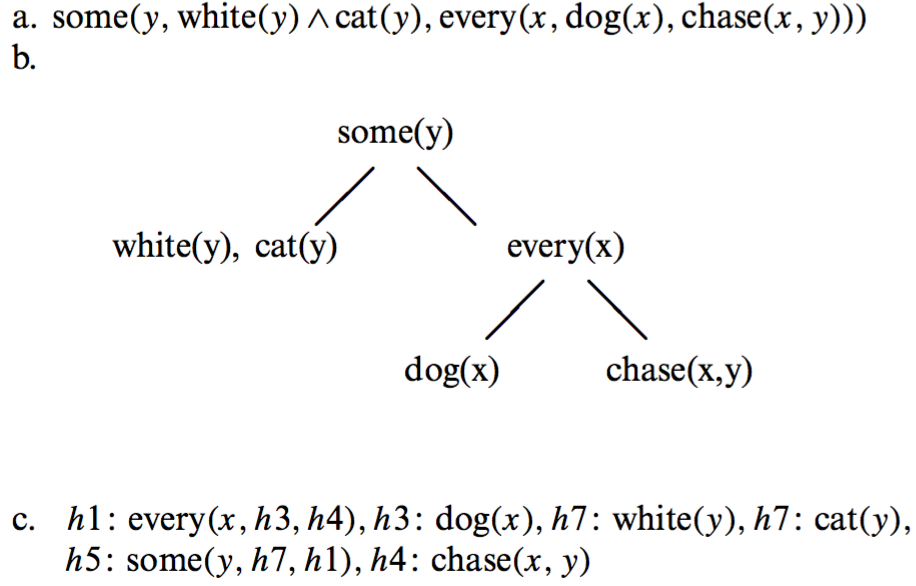
\includegraphics[height=4cm,width=6cm]{img/parse01.png}
            
            \column{0.5\textwidth}
            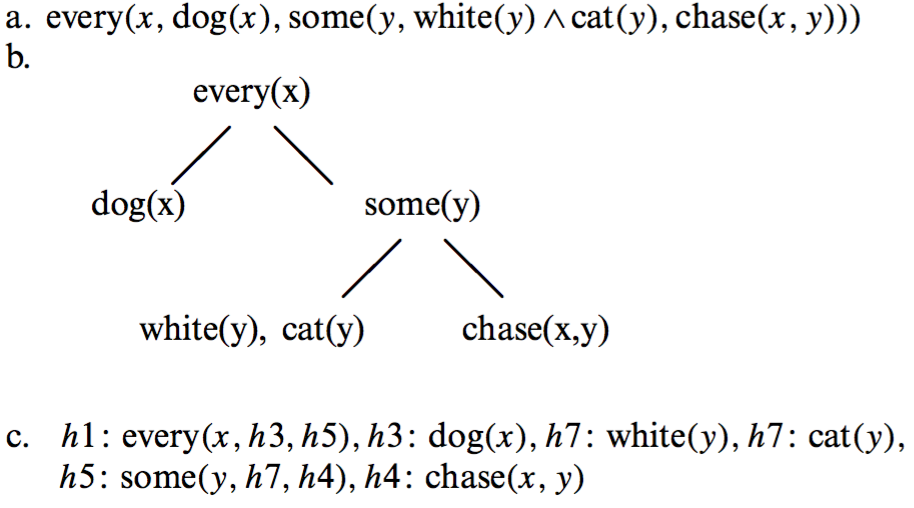
\includegraphics[height=4cm,width=6.3cm]{img/parse02.png}
        \end{columns}
    }

    \only<2>{
        \begin{columns}
            \column{0.7\textwidth}

            Leave some handles unspecified.

            \begin{itemize}

                \item Then specify it later: $h0 = h1, h3 = h5, h7 = h4$

                \item constraints, $h3 \neq h7$ to make it still a tree

                \item qeq constraint, $h0 =_q h5$ is a trival example

            \end{itemize}

            \column{0.3\textwidth}

            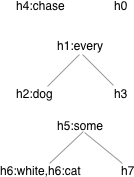
\includegraphics[height=4cm]{img/unresolved-parse.png}

        \end{columns}
    }

\end{frame}

\begin{frame}
    \frametitle{MRS formally in a whole}

    MRS is a quadruple \{GT, LT, R, C\}

    \begin{itemize}
        \item GT: global top. h0
        \item LT: local top. h1, h4, h5 (semantic of local phrase)
        \item R: relations. h1:every(x, h2, h3), h5:dog(y, h6, h7), h4:chase(x), etc.
        \item C: constraints. h0 qeq h4, etc.
    \end{itemize}
\end{frame}

\begin{frame}
    \frametitle{Highlights of MRS}

    \begin{itemize}
        \item We reify scopal relationships as handles
            so that syntactically the language looks first-order.
        \item Preserve \emph{underspecifiability}
    \end{itemize}
\end{frame}

\subsection{AMR}

\begin{frame}
    \frametitle{Abstract Meaning Representation (Banarescu, 2013)}

    AMR is an semantic representation that

    \begin{itemize}
        \item is rooted, directed and labeled graph
        \item is identical for different utterance
        \item uses variables for co-reference
        \item uses PropBank frame (analogous to roles in neo-Davidsonian)
        \item designs non-core relations out of PropBank
            (analogous to adjuncts in neo-Davidsonian)
    \end{itemize}

    Specification: https://github.com/amrisi/amr-guidelines/blob/master/amr.md

\end{frame}

\begin{frame}[fragile] % fragile is for verbatim
    \frametitle{An AMR Example}

    \emph{Brutus stabbed Caesar with a knife in the back in the agora and twisted it hard.}

    \begin{verbatim}
(s / stab
      :ARG0 (p / person :name (n / name :op1 "Brutus")
            :ARG0-of (t / twist
                  :ARG1 k
                  :manner (h / hard)))
      :ARG1 (p2 / person :name (n2 / name :op1 "Caesar"))
      :ARG2 (k / knife)
      :ARG3 (b / back)
      :location (a / agora))
    \end{verbatim}
\end{frame}

\begin{frame}[fragile]
    \frametitle{Event Frames Rise from Various POS}

    \begin{itemize}
        \item Verb \pause
        \item Noun

            \begin{examples}
            \emph{the destruction of the city by the God}
            \begin{verbatim} (d / destroy-01 :ARG0 (g / God) :ARG1 (c / city)) \end{verbatim}
            \end{examples}

            \begin{examples}
            \emph{the bond investor}
            \begin{verbatim} (p / person :ARG0-of (i / invest-01 :ARG1 (b / bond))) \end{verbatim}
            \end{examples}

            \only<2>{but \emph{professor} doesn't yield an event frame}

            \pause

        \item Adjective

            \begin{examples}
            \emph{the attractive spy}
            \begin{verbatim} (s / spy :ARG0-of (a / attract-01)) \end{verbatim}
            \end{examples}
    \end{itemize}
\end{frame}

\begin{frame}[fragile]
    \frametitle{Reification - Frame from Non-Core Relation}

    An adjunct for non-core relation in AMR must serve as a role for the relation,
    rather than for any object participating in that relation.

    \begin{examples}
    \emph{the marble in the jar}
    \begin{verbatim} (m / marble :location (j / jar)) \end{verbatim}

    \emph{the marble is not in the jar}
    \begin{verbatim} (b / be-located-at-91
    :ARG1 (m / marble) :ARG2 (j / jar) :polarity -) \end{verbatim}
    \end{examples}

    \begin{alertblock}{Semantic Error}
    \begin{verbatim} (m / marble :location (j / jar :polarity -)) \end{verbatim}
    which reads \emph{the marble is in the non-jar}
    \end{alertblock}
\end{frame}

\begin{frame}
    \frametitle{Other Language Phenomenons Defined in AMR}

    AMR defines approximately 100 relations for language phenomenons.

    \begin{itemize}
        \item negation and modals
        \item interrogation and wh-questions
        \item named entities
        \item location source, destination, path
        \item cause, concession, condition
        \item quantities, date, time
        \item link with wikipedia article :wiki ``Barack\_Obama''
        \item \dots
    \end{itemize}

\end{frame}

\begin{frame}
    \frametitle{AMR Data Overview}

    1. Annotated Corpus:

    \begin{itemize}
        \item \emph{The Little Prince}, 1274:145:143
        \item \emph{The Little Prince} Chinese Version, 1274:145:143
        \item Bio AMR Corpus from PubMed (cancer) articles, 5452:500:500
        \item LDC Corpus General Release 1.0 (June 2014), 13051 in all, \\
            a new general release is due in summer of 2016
    \end{itemize}

    2. Evaluation: smatch metric, comparison of two AMR

    3. SemEval-2017 Task 9: Parsing and Generation

    \begin{itemize}
        \item English Biomedical Data to AMR (SemEval-2016 Task 8)
        \item AMR to English Generation
    \end{itemize}

    4. A python parser: https://github.com/nschneid/amr-hackathon

\end{frame}
\begin{frame}
    \frametitle{Chinese AMR Corpus Example}

    \begin{center}
        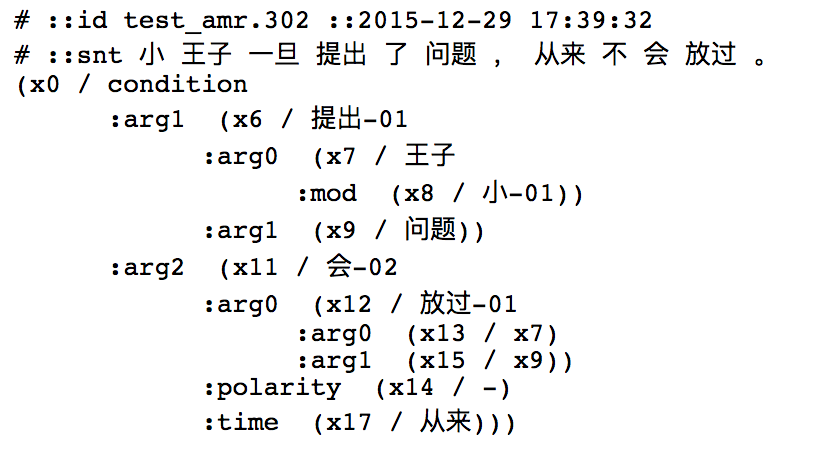
\includegraphics[height=7cm,width=12cm]{img/little-prince-chn-parse.png}
    \end{center}
\end{frame}

\begin{frame}
    \frametitle{AMR Editor}

    A simple web editor to build an AMR.

    \begin{center}
        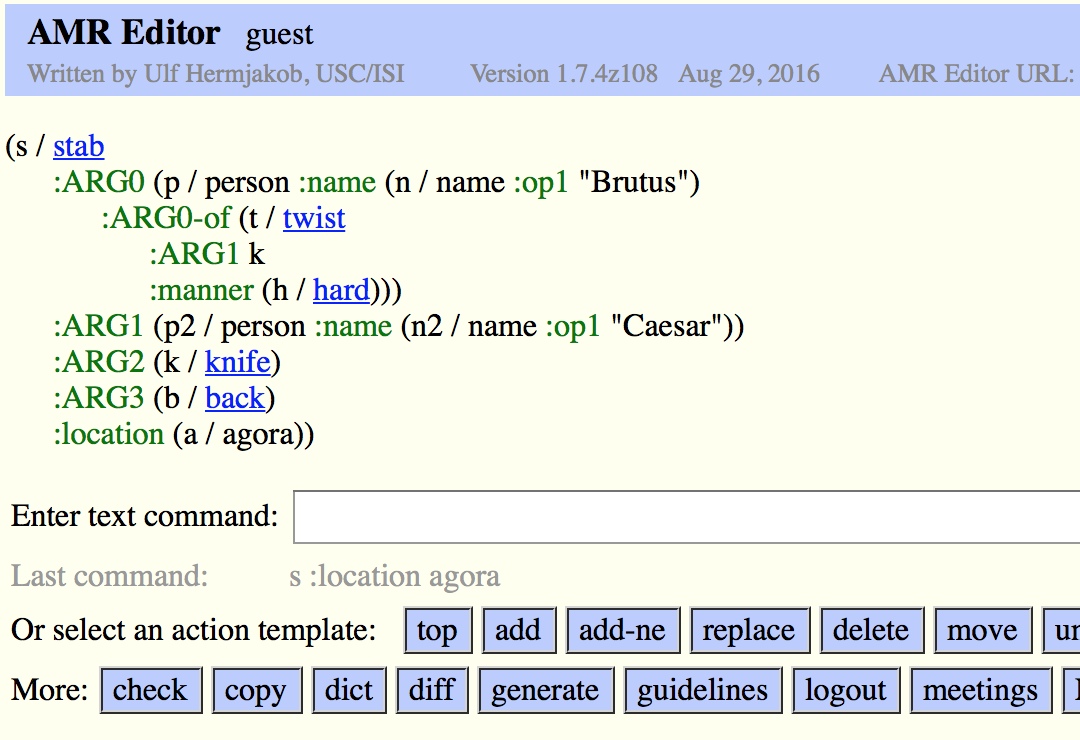
\includegraphics[height=6.7cm,width=9.8cm]{img/amr-editor.png}
    \end{center}
\end{frame}

\section{Parsing}

\begin{frame}
    \frametitle{Parsing Methods}

    There're many semantic parsing paradigms.

    Some of them are new methods while others borrow ideas from other domains or tasks to do semantic parsing exactly.

    \begin{itemize}
        \item Shift-Reduce (LR) (1993)
        \item Combinatory Categorial Grammar (2005)
        \item Word Alignment (Synchronized CFG) (2006)
        \item Generative Model (2008)
        \item Syntactic Parse to Semantic Parse (2009)
        \item Weak Supervision and Unsupervised Methods (2010)
        \item Large-scale SP for Freebase and QA (2013)
        \item Paraphrase-driven SP (2014)
        \item Neural Semantic Parsing (2015)
    \end{itemize}

\end{frame}

\subsection{Shift-Reduce}

\begin{frame}
    \frametitle{Inductive Logic Programming (Zelle et al., 1993)}

    Shift-Reduce is a simple bottom-up parsing. 

    \begin{center}
        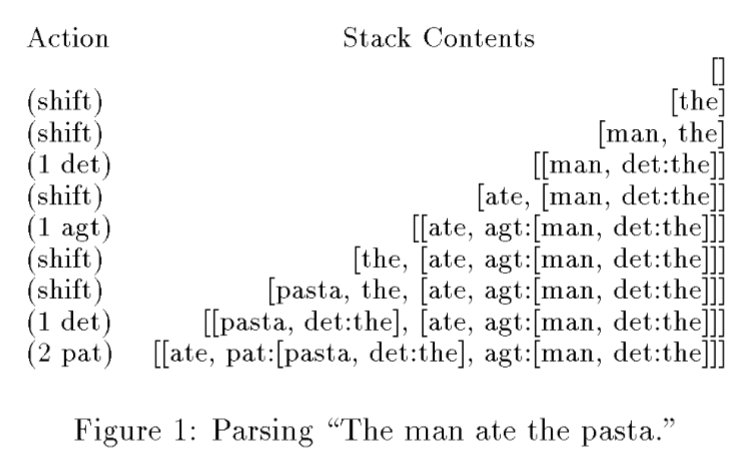
\includegraphics[height=4.62cm,width=7.55cm]{img/shift-reduce.png}
    \end{center}

    Each action correspond to a prolog clause.
    \begin{center}
        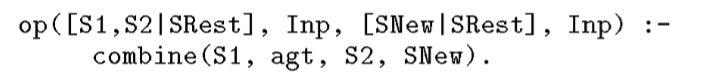
\includegraphics[height=0.6cm,width=6cm]{img/prolog-clause.png}
    \end{center}
\end{frame}

\begin{frame}
    \frametitle{Inductive Logic Programming (Zelle et al., 1993)}

    CHILL(Constructive Heuristic Induction for Language Learning)

    \begin{itemize}
        \item Find\_Generalization: merge clauses not cover any negative sample.
        \item Reduce\_Definition: prefer new clause to prove positive examples
    \end{itemize}

    \begin{center}
        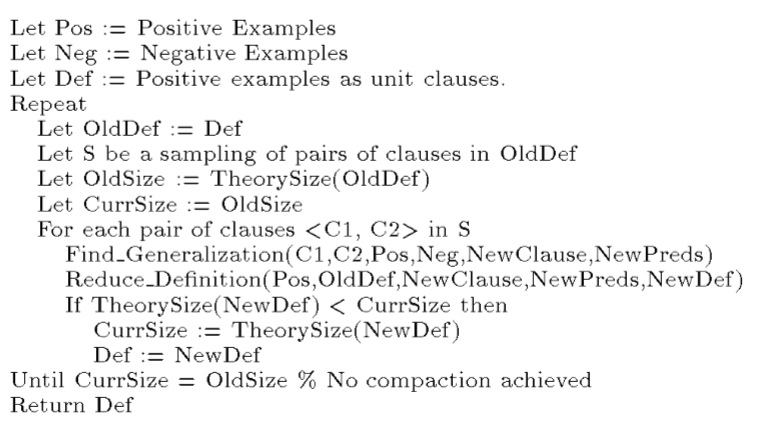
\includegraphics[height=6.5cm,width=10cm]{img/inductive-logic.png}
    \end{center}
\end{frame}

\begin{frame}
    \frametitle{CHILL on GeoQuery (Zelle et al., 1996)}

    \only<1>{
        \begin{columns}
            \column{0.5\textwidth}
            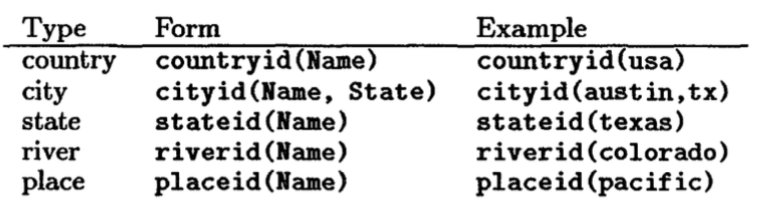
\includegraphics[height=1.7cm,width=5cm]{img/geoquery-object.png}

            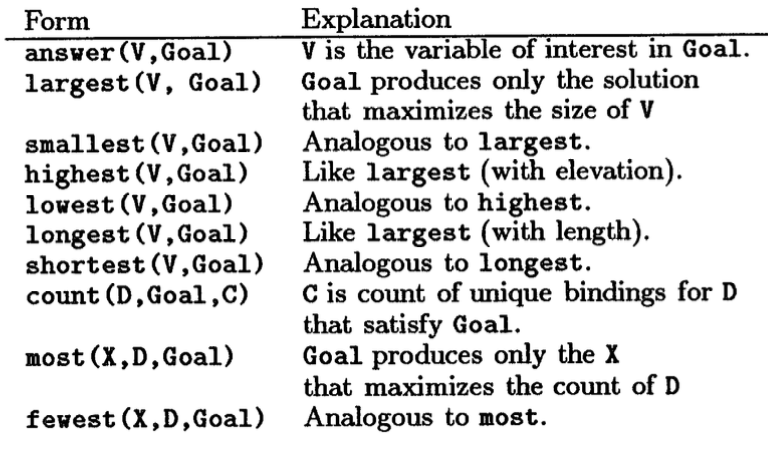
\includegraphics[height=4.5cm,width=6cm]{img/geoquery-meta-predicate.png}

            \column{0.5\textwidth}
            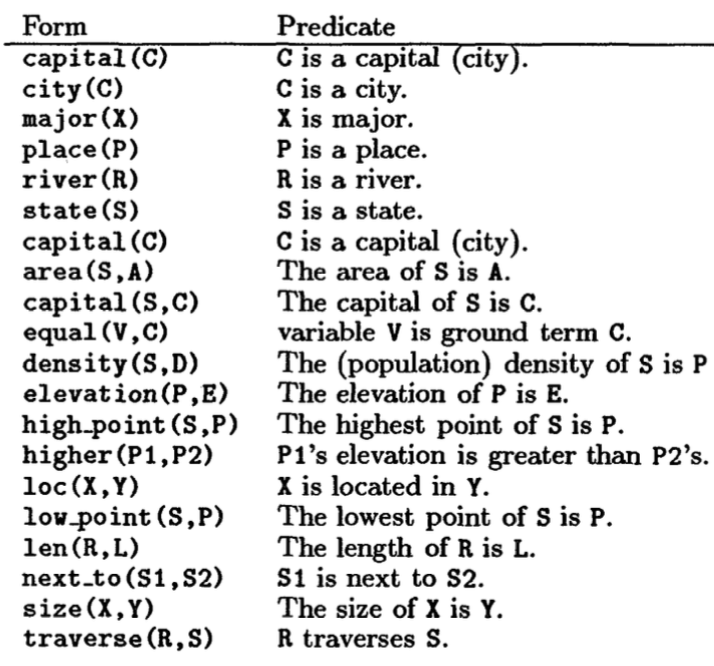
\includegraphics[height=6.5cm,width=6cm]{img/geoquery-predicate.png}
        \end{columns}
    }

    \only<2> {
        \begin{center}
            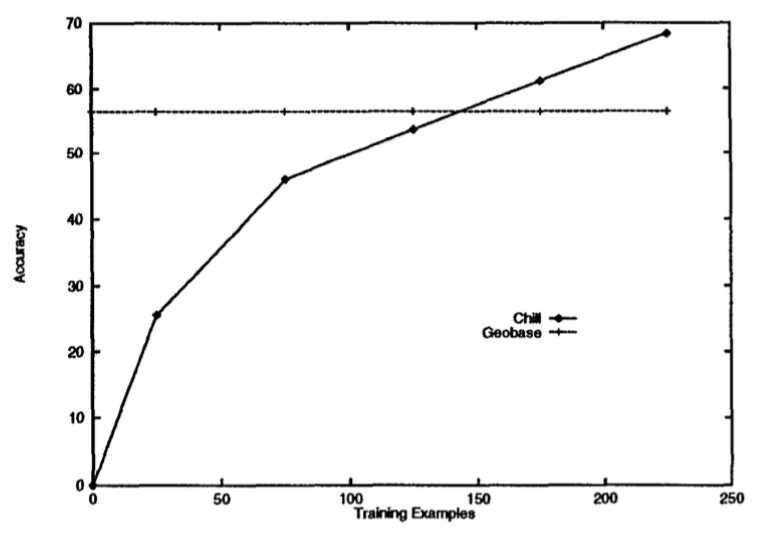
\includegraphics[height=8cm,width=10cm]{img/chill-geoquery-acc.png}
        \end{center}
    }
\end{frame}

\subsection{CCG}

\begin{frame}
    \frametitle{Combinatory Category Grammar (Steedman, 1996, 2000)}

    \only<1> {
        CCG comes with a lexicon whose element is a pair of word and a category:

        \[
            \text{borders} := (S \backslash NP) / NP : \lambda x . \lambda y . borders(y, x)
        \]

        \begin{itemize}
            \item word: $borders$
            \item syntactic type: $(S \backslash NP) / NP$
            \item semantic type: $\lambda x . \lambda y . borders(y, x)$
        \end{itemize}
    }

    \only<2> {
        Categories can be combined.

        \begin{itemize}
            \item forward and backward application

                \begin{tabular}{rlrl}
                    A / B : f &+  &B : x        &$\Rightarrow$ A : f(x) \\
                        B : x &+  &A $\backslash$ B : f &$\Rightarrow$ A : f(x)
                \end{tabular}

            \item forward and backword composition

                \begin{tabular}{rlrl}
                    A / B : f &+  &B / C : g   &$\Rightarrow$ A / C : $f\circ g$  \\
                    A $\backslash$ B : f &+  &B $\backslash$ C : g &$\Rightarrow$
                        A $\backslash$ C : $f\circ g$  \\
                \end{tabular}

            \item type raising

                $X \Rightarrow T / (T \backslash X)$

        \end{itemize}
    }

    \only<3> {
        A CCG Parse Example.

        \begin{center}
            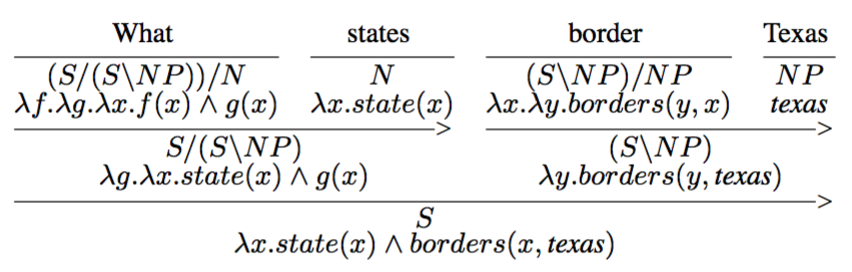
\includegraphics[height=2.72cm,width=8.52cm]{img/ccg-parse.png}
        \end{center}
    }
\end{frame}

\begin{frame}
    \frametitle{Semantic Parsing using CCG on GeoQuery}
    \framesubtitle{Zettlemoyer and Collins, 2005}

    Given the lexicon and model parameter, CCG is formulated as a log-linear probablistic model
    to deal with ambiguity,
    e.g. duplicated lexicon entries for a word, and spurious ambiguity:

    \[
        P(L, T \mid S; \bar\theta) = \frac
            {\exp(\bar f(L,T,S)\cdot\bar\theta)}
            {\sum_{(L,T)}\exp(\bar f(L,T,S)\cdot\bar\theta)}
    \]

    And we can do inference on the model:

    \[
        L = \arg\max_L P(L\mid S;\bar\theta) = \arg\max_L\sum_TP(L,T\mid S;\bar\theta)
    \]

    Features are designed as local and thus we can use dynamic programming
    (beam-search acturally) and prune the search space (like CKY-style).

\end{frame}

\begin{frame}
    \frametitle{Learning the Model (Zettlemoyer et al. 2005)}

    Learning the parameters using SGD.

    \begin{center}
        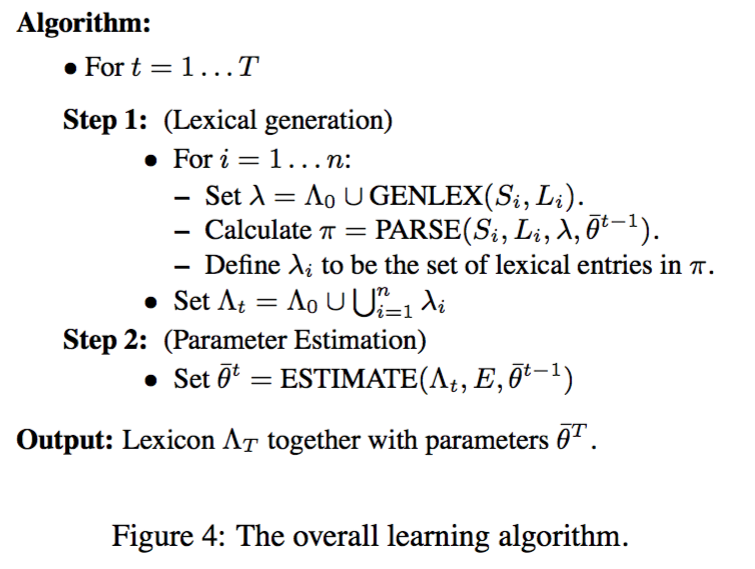
\includegraphics[height=5.69cm,width=7.55cm]{img/learning-algo.png}
    \end{center}

\end{frame}

\begin{frame}
    \frametitle{Learning the Lexicon (Zettlemoyer et al. 2005)}

    \[
        GENLEX(S,L) = \{x := y \mid x \in W(S), y\in C(L)\}
    \]

    \begin{itemize}
        \item W(S) is all subsequence of S
        \item C(L) produces categories using rules L triggered
    \end{itemize}

    \begin{center}
        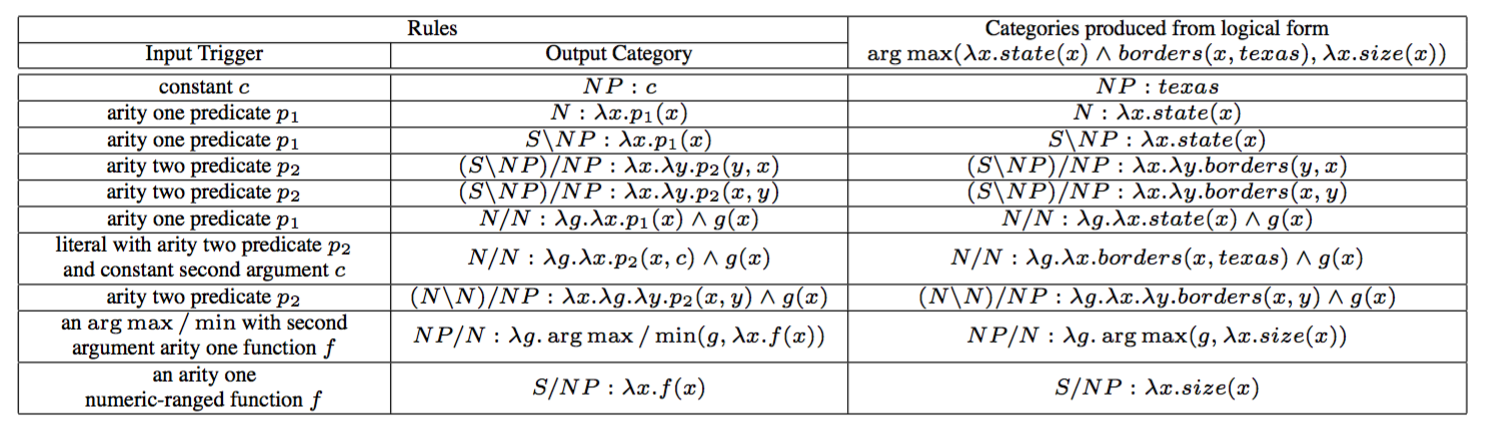
\includegraphics[height=5.32cm,width=12cm]{img/zc05-triggers.png}
    \end{center}

\end{frame}

\begin{frame}
    \frametitle{Problems in ZC05}

    GENLEX is controlled by rules, and will be insufficient
    if the rules don't cover all the (S, L) pairs.

    \begin{examples}
    Through which states does the Mississippi run.
    \end{examples}

    GENLEX doesn't trigger a category suitable for the \emph{through}-adjunct placed ahead.

    Namely, phrase order may be relaxed.
\end{frame}

\begin{frame}
    \frametitle{Relaxed Combinatory Rules (Zettlemoyer et al., 2007)}

    \begin{itemize}
        \item relaxed function application

            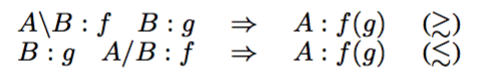
\includegraphics[height=1cm,width=5cm]{img/ccg-relax-01.png}

        \item relaxed function composition

            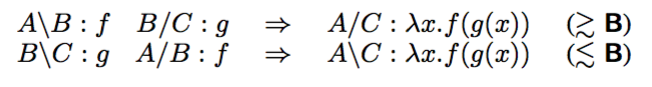
\includegraphics[height=1cm,width=6.5cm]{img/ccg-relax-02.png}

        \item role-hypothesising type shifting (for missing predicates)

            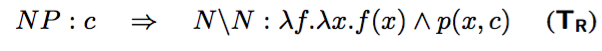
\includegraphics[height=0.6cm,width=6cm]{img/ccg-relax-03.png}

        \item null-head type shifting (for missing arguments)

            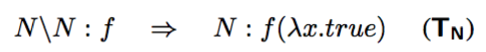
\includegraphics[height=0.6cm,width=5cm]{img/ccg-relax-04.png}

        \item crossed functional composition

            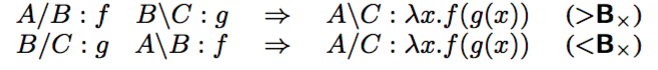
\includegraphics[height=0.8cm,width=6.5cm]{img/ccg-relax-05.png}
    \end{itemize}

    Triggers are added for these new rules, too.

\end{frame}

\begin{frame}
    \frametitle{Online Learning (Zettlemoyer et al., 2007)}

    Use a peceptron learning instead. New features are also added.

    \begin{center}
        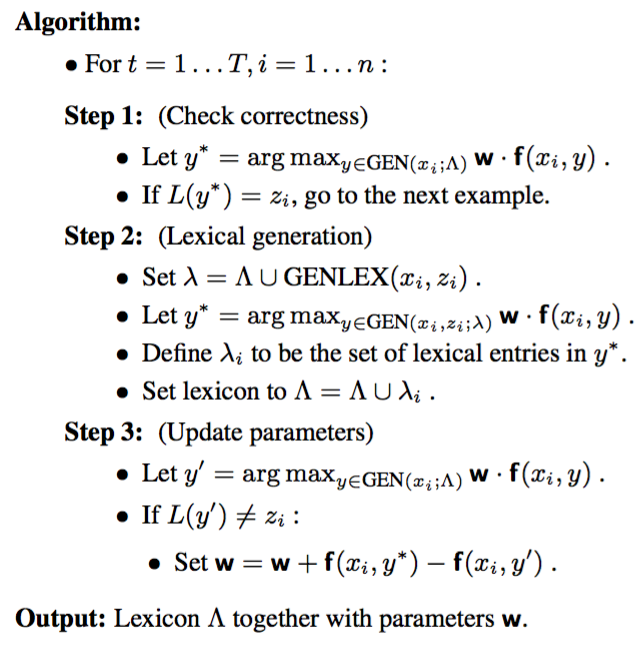
\includegraphics[height=6.5cm,width=6.42cm]{img/zc07-learn-02.png}
    \end{center}
\end{frame}

\begin{frame}
    \frametitle{Problems in ZC07}

    GENLEX needs hand-written rules.
\end{frame}

\begin{frame}
    \frametitle{CCG Induction using Unification (Kwiatkowski et al. 2010)}

    Unification in wikipedia:

    \begin{quotation}
        Unification is an algorithmic process of solving equations between symbolic expressions.
        e.g.
        $\{ cons(x,cons(x,nil)) = cons(2,y) \} \Rightarrow \{  x \to 2, y \to cons(2,nil) \}$
    \end{quotation}

    Here \emph{unification} aims to {\color[rgb]{0,0,1}find f and g given h}, s.t.
    \begin{center}
        $h = \lambda x. f(g(x))$ or $h = f(g)$.
    \end{center} \pause

    For example, the given initial lexical entry
    \[
        \text{New York borders Vermont} \vdash S: next\mathunderscore to(ny, vt)
    \]

    will be splitted as 
    \begin{align*}
        \text{New York borders} &\vdash S / NP : \lambda x . next\_to(ny, vt) \\
        \text{Vermont}          &\vdash NP : vt
    \end{align*}

\end{frame}

\begin{frame}
    \frametitle{CCG Induction using Unification (Kwiatkowski et al. 2010)}

    \only<1> {
        Parsing with PCCG
        \begin{align*}
            P(y, z \mid x; \theta, \Lambda) = \frac{\exp(\theta\cdot\phi(x,y,z))}{Z(y',z')} \\
            f(x) = \arg\max_z p(z\mid x; \theta, \Lambda) \\
            p(z \mid x; \theta, \Lambda) = \sum_y p(y, z \mid x; \theta, \Lambda)
        \end{align*}

        Again, to compute the parse efficiently, 
        \begin{itemize}
            \item CKY-style parsing with dynamic programming
            \item summing over y with inside-outside algorithm
        \end{itemize}
    }

    \only<2> {
        Learning algorithm: NEW-LEX will consider whether to split the lexical entries
        and gives new lexicon from $\arg\max_{y^*}p(y^*\mid x_i, z_i; \theta', \Lambda')$
        \begin{center}
            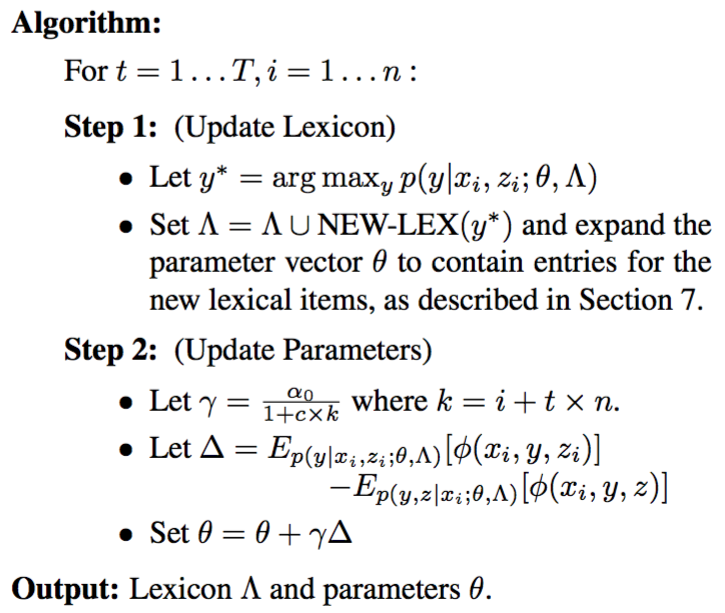
\includegraphics[width=7.25cm,height=6.13cm]{img/unification-learning.png}
        \end{center}
    }

\end{frame}

\begin{frame}
    \frametitle{Split a lexicon (Kwiatkowski et al. 2010)}

    Split a lexical entry: Step 1, function
    \[
        \text{New York borders Vermont} \vdash S: \textcolor{red}{next\_to(ny, vt)}
    \]

    unification constraints (otherwise infinite-result):
    \begin{itemize}
        \item No vacuous variables: $g \ne \lambda x . tex$
        \item limited coordination extraction: $g$ contains less than N adjuncts
        \item limited application: $f$ contains no new variables for non-variable
            subexpression in $h$ like 
            \begin{align*}
                h &= \lambda x . in(x, tex) \\
                f &\to \lambda q . q(tex) \\
                g &\to \lambda y \lambda x . in(x, y)
            \end{align*}
    \end{itemize}

    \pause

    we can get many (f, g) pairs, among which there is: 
    \[
        f \to \lambda x . next\_to(ny, x)\,\,\,\,\, g \to vt
    \]
\end{frame}

\begin{frame}
    \frametitle{Split a lexicon (Kwiatkowski et al. 2010)}

    Split a lexical entry: Step 2, syntactic type
    \[
        \text{New York borders Vermont} \vdash \textcolor{red}{S}: next\_to(ny, vt)
    \]

    \only<1> {
        According to CCG combinatory rules(only 4 here), define
        \begin{align*}
            S_C(A) &= \{FA(A) \cup BA(A) \cup FC(A) \cup BC(A) \}\\
            FA(X:h)&= \{ (X / Y : f, Y : g) \mid h = f(g) \wedge Y = C(T(g)) \}  \\
            BA(X:h)&= \{ (Y : g, X \backslash Y : f) \mid h = f(g) \wedge Y = C(T(g)) \}  \\
            FC(X / Y:h)&= \{ (X / W : f, W / Y : g) \mid
                h = \lambda x . f(g(x)) \wedge W = C(T(g(x))) \}  \\
            BC(X \backslash Y:h)&= \{ (W \backslash Y : f, X \backslash W : g) \mid
                h = \lambda x . f(g(x)) \wedge W = C(T(g(x))) \}
        \end{align*}
        where $T: F \to \{e, t, F\}$ is the type function and C is defined as
        \begin{gather*}
            C(T) = \begin{cases}
                NP & \text{ if } T=e \\ 
                S & \text{ if } T=t \\ 
                C(T_2)\vert C(T_1)  & \text{ if } T= \langle T_1, T_2\rangle
            \end{cases}
        \end{gather*}
    }

    \only<2> {
        These are some possible pair from the splitting set.
        \begin{itemize}
            \item Semantic: \textcolor{blue}{$(\lambda x . next\_to(ny, x), vt)$}

                Syntactic: $(S/NP, NP)$

            \item Semantic: \textcolor{blue}{$(ny, \lambda x . next\_to(x, vt))$}

                Syntactic: $(NP, S\backslash NP)$

            \item Semantic: \textcolor{red}{$(\lambda x . next\_to(x, vt), ny)$}

                Syntactic: $(S/NP, NP)$

        \end{itemize}
    }

\end{frame}

\begin{frame}
    \frametitle{Split a lexicon (Kwiatkowski et al. 2010)}

    Split a lexical entry: Step 3, word sequence
    \[
        \textcolor{red}{\text{New York borders Vermont}} \vdash S: next\_to(ny, vt)
    \]
    Splitting is defined as
    \[
        S_L(w_{0:n}\vdash A) = \{(w_{0:i}\vdash B, w_{i+1:n}\vdash C) \mid
            0 \leq i < n \wedge (B, C) \in S_C(A) \}
    \] \pause
    For some specific i, the previous splits may raise problems.
    \begin{itemize}
        \item \textcolor{blue}{$(S/NP:\lambda x . next\_to(ny, x), NP:vt)$}

            Sequence: (New York borders, Vermont)

        \item \textcolor{blue}{$(NP:ny, S\backslash NP:\lambda x . next\_to(x, vt))$}

            Sequence: (New York, borders Vermont)

        \item \textcolor{red}{$(S/NP:\lambda x . next\_to(x, vt), NP:ny)$}

            Sequence: (borders Vermont, New York) incorrect

    \end{itemize}

\end{frame}

\begin{frame}
    \frametitle{Problems in Kwiatkowski et al. 2010}

    Learned CCG lexicon is too big.
\end{frame}

\begin{frame}
    \frametitle{Factored Lexicon in CCG (Kwiatkowski et al 2011)}

    Original lexical entry: $Boston \vdash N / N:\lambda f\lambda x.from(x, bos) \wedge f(x)$

    Factored Parts:
    \begin{itemize}
        \item lexeme, pair of a word span and a constant list: $(Boston,[from,bos])$
        \item template, $\lambda (w, \vec v).(w \vdash N / N:\lambda f\lambda x.v_1(x, v_2) \wedge f(x))$
    \end{itemize}

    \pause

    Two type of factorization:
    \begin{enumerate}
        \item maximal factor: all constants are in lexeme

            $(Boston, [from, bos]),  
            \lambda (w, \vec v).(w \vdash N / N:\lambda f\lambda x.v_1(x, v_2) \wedge f(x))$

        \item partial factor: some constants remain in the template
            $(Boston, [bos]), 
            \lambda (w, \vec v).(w \vdash N / N:\lambda f\lambda x.from(x, v_1) \wedge f(x))$

            Partial factor is used for missing words: \emph{flights Boston to New York}
    \end{enumerate}

\end{frame}

\begin{frame}
    \frametitle{Factored Lexicon in CCG (Kwiatkowski et al 2011)}

    Learning is similar but to consider factorization:

    \begin{center}
        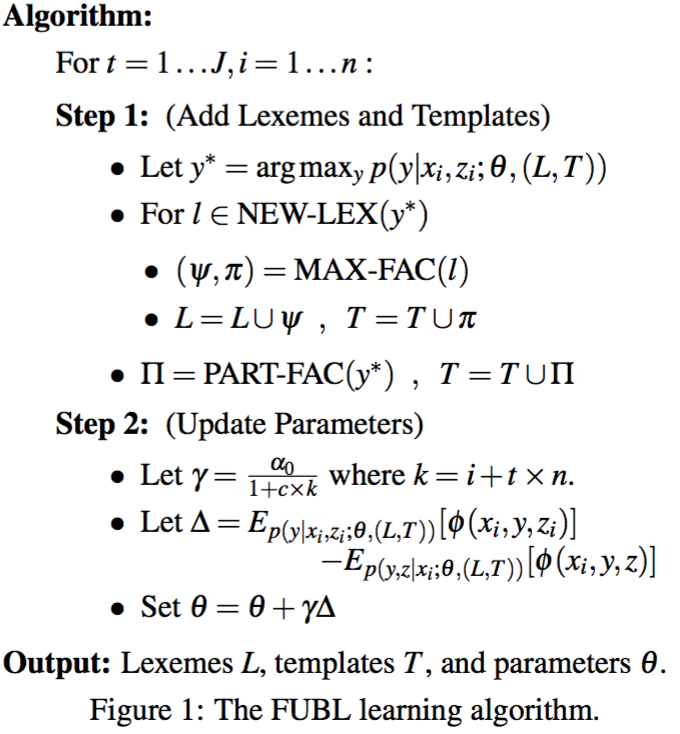
\includegraphics[width=6.8cm,height=7.34cm]{img/fubl.png}
    \end{center}

\end{frame}

\begin{frame}
    \frametitle{Problems in Kwiatkowski et al. 2011}

    Learned CCG lexicon is too big.
\end{frame}

\begin{frame}
    \frametitle{test}
\end{frame}

\begin{frame}
    \frametitle{test}
\end{frame}

\begin{frame}
    \frametitle{test}
\end{frame}

\begin{frame}
    \frametitle{test}
\end{frame}

\begin{frame}
    \frametitle{test}
\end{frame}

\end{document}
